%!TEX root = draft.tex

\section{Convergent Return-Value Consistency}
\label{sec:specifications and consistencies}

%In this section, we introduce our formation of specification. Then, we propose strong-return-value consistency, which is a sub-notion of eventual consistency of \cite{Bouajjani:2014} that strengthen the ``safety part'' specific for intuition of CRDT algorithms and ignores the ``liveness part''.




%\subsection{Specification}
%\label{subsec:specification}

%Given

%\begin{itemize}
%\setlength{\itemsep}{0.5pt}
%\item[-] $\mathbb{M}$ be a finite set of method names,

%\item[-] $\mathbb{D}$ be a possibly infinite set of data domain for argument and return values,

%\item[-] $\mathbb{R}$ be a finite set of replica identifiers, and

%\item[-] $\mathbb{O}$ be a infinite set of operation identifiers.
%\end{itemize}

%\todo{Define ``operation label'' which is $m(a,b)$ and denote operation labels by $\ell$. Operation content is not a good name.}

Given a finite set $\mathbb{M}$ of method names, a possibly infinite set $\mathbb{D}$ of data domain for argument and return values, a finite set $\mathbb{R}$ of replica identifiers, and a infinite set $\mathbb{O}$ of operation identifiers. A operation label is a tuple $m(a)\Rightarrow b$ where $m \in \mathbb{M}$ and $a,b \in \mathbb{D}$. $m(a) \Rightarrow b$ represents that $m$ is called with argument $a$ and returns b. When $m$ does not use the argument (resp., return value), we write $m()\Rightarrow b$ (resp., $m(a)$) instead. An operation $o$ is a tuple $(\ell,r,i)$, where $\ell$ is a operation label, $r \in \mathbb{R},i \in \mathbb{O}$. Let $\mathit{lab}(o)$ be the operation label of $o$. This definition extends naturally to the case when there are more than one arguments. Methods of $\mathbb{M}$ can be divided into query methods with names in $\mathbb{Q}$ and update methods with names in $\mathbb{U}$.

{\color {red}We use the notion of history to capture the user-observable behaviors, which contains operations and their order on each replica.} A history is a tuple $(O,\mathit{ro})$, where $O$ is a set of operations, and $\mathit{ro}$ is called the replica order. For each replica $r \in \mathbb{R}$, $\mathit{ro}$ is a irreflexive total order over operations with replica identifier $r$. $\mathit{ro}$ does not relate operations with different replica identifiers. %We also require that for each operation $o \in O$, $\mathit{ro}^{-1}(o)$ is finite.
{\color {red}An example of distributed list history is shown in \figurename~\ref{fig:history, annotated history and operation context} (a).}

%CRDT has two kinds of method: query methods and update methods.
{\color{red}To check the correctness of a history, we augment it with additional information to explain the observed operations. In this way we obtain annotated history.} An annotated history is a tuple $(O,\mathit{vis},\mathit{arb})$, where $O$ is a set of operations, $\mathit{vis}$ is called the visibility relation and is a irreflexive and acyclic relation over $O$ , and $\mathit{arb}$ is called the arbitration order and is a irreflexive total order over a subset of update operations of $O$. {\color {red} Visibility relation tells how update operations are delivered, and arbitration order represents some global orders that are used to determine return values on each replica, such as list order in \cite{Attiya:2016} or time stamp order.} We further require that for each operation $o \in O$, $\mathit{vis}^{-1}(o)$ is finite. {\color {red}The annotated history for history of \figurename~\ref{fig:history, annotated history and operation context} (a) is given in \figurename~\ref{fig:history, annotated history and operation context} (b).} % with arbitration order $\mathit{add}(b,1) \cdot \mathit{add}(c,2) \cdot \mathit{add}(a,1)$.}

%\begin{itemize}
%\setlength{\itemsep}{0.5pt}
%\item[-] $O$ is a set of operations.

%\item[-] $\mathit{vis}$ is a irreflexive and acyclic relation over $O$, and is called the visibility relation. We require that for each operation $o \in O$, $\mathit{vis}^{-1}(o)$ is finite.

%\item[-] $\mathit{arb}$ is a partial order over update operations of $O$ and is called the arbitration order.
%\item[-] $\mathit{arb}$ is a irreflexive total order over a subset of update operations of $O$ and is called the arbitration order.
%\end{itemize}


\begin{figure}[t]
  \centering
  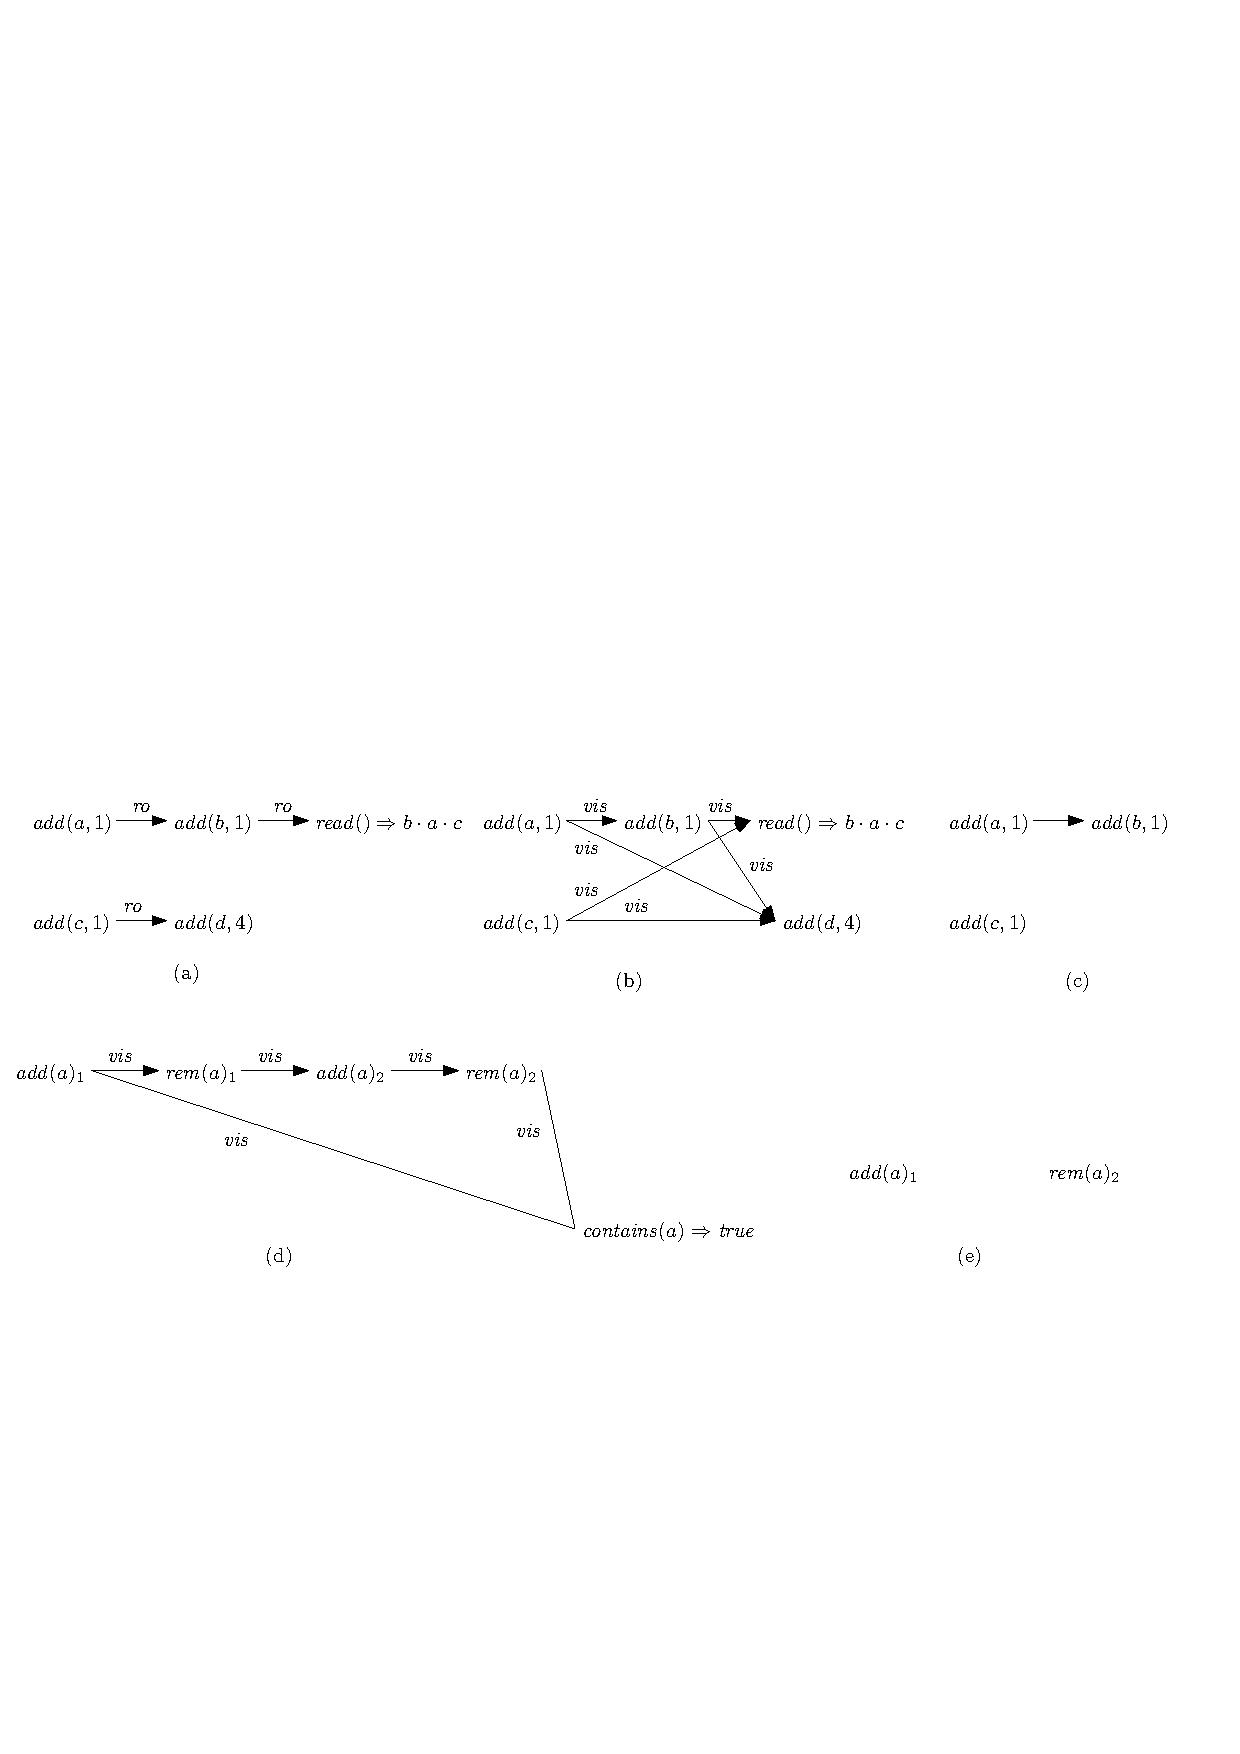
\includegraphics[width=0.75 \textwidth]{figures/PIC-his-anhis-context.pdf}
%\vspace{-10pt}
  \caption{History, its annotated history and operation context. Here $+(a,1)$ represents $\mathit{add}(a,1)$, $r(b \cdot a \cdot c)$ represents $\mathit{read}(b \cdot a \cdot c)$; $+a_1$ and $-a_1$ represents $\mathit{add}(a)$ and $\mathit{rem}(a)$, respectively, while the subscript number is used to distinguish different $\mathit{add(a)}$; $(a,\surd)$ represents $\mathit{contains}(a,\mathit{true})$. In annotated history (b), we use arbitration order $\mathit{add}(b,1) \cdot \mathit{add}(a,1) \cdot \mathit{add}(c,1) \cdot \mathit{add}(d,4)$. Assume that the visibility relation contains the replica order.}
  \label{fig:history, annotated history and operation context}
\end{figure}


{\color {red}Similarly as in \cite{Burckhardt:2014}, in defining specification, we use the notion of operation context, which contains all information necessary to ensure the correctness of an operation.} A operation context of a operation $o$ is a tuple $(O,<,\mathit{arb})$, where $O$ is a set of update operations, $<$ is a relation over $O$, $o \notin O$, and $\mathit{arb}$ is a irreflexive total order over a subset of update operations of $O \cup \{ o \}$. {\color {red}Here we modified that of \cite{Burckhardt:2014} by making $o \notin O$ itself also contained in the arbitration order. This feature is used to deal with list specification.} A specification $\mathit{Spec}$ is a function that maps each operation label $\ell$ into a set of elements, while each of them is a operation context $(O,<,\mathit{arb})$ for some operation $o$ with $\mathit{lab}(o) = \ell$. {\color {red} For example, \figurename~\ref{fig:history, annotated history and operation context} (c) is in specification of $o = \mathit{add}(d,4)$.} A specification is deterministic, if there does not exists query method $m$ and tuple $(O,<,\mathit{arb})$, such that $(O,<,\mathit{arb})$ is in both $\mathit{Spec}(m(a) \Rightarrow b)$ and $\mathit{Spec}(m(a') \Rightarrow b')$, and $a \neq a' \vee b \neq b'$. From now on, we consider only deterministic specifications.

Given an annotated history $(O,\mathit{vis},\mathit{arb})$ and an operation $o \in O$, the operation context of $o$ is a obtained by a tuple $ctxt(o)=(O',<,\mathit{arb}')$, where $O'$ is the set of update operations in $\mathit{vis}^{-1}(o)$, $<$ is the projection of $\mathit{vis}$ over $O'$, and $\mathit{arb}'$ is the projection of $\mathit{arb}$ over update operations of $O' \cup \{ o \}$. Therefore, given an annotated history $(O,\mathit{vis},\mathit{arb})$ and $o_1,o_2 \in O$, if $o_1$ and $o_2$ see the same set of operations, %$\mathit{vis}^{-1}(o_1) = \mathit{vis}^{-1}(o_2)$,
then $O_1 = O_2$ and $<_1 = <_2$, where $ctxt(o_1)=(O_1,<_1,\mathit{arb}_1)$ and $ctxt(o_2)=(O_2,<_2,\mathit{arb}_2)$. This comply with the commutativity intuition of CRDT algorithm. {\color {red} For example, \figurename~\ref{fig:history, annotated history and operation context} (c) is also the operation context of $o = \mathit{add}(d,4)$ in \figurename~\ref{fig:history, annotated history and operation context} (b).} {\color {red}Similarly, this definition modifies that of \cite{Burckhardt:2014} to deal with list.} Note that the uniformly method of obtaining operation context from annotated history is suitable for most specifications. For one special case, the OR-set, we shows how to deal with it in Remark \ref{remark: operation context of OR-set}.

%To comply with the commutativity intuition of CRDT algorithm, we further require that, given an annotated history $(O,\mathit{vis},\mathit{arb})$ and $o_1,o_2 \in O$, if $\mathit{vis}^{-1}(o_1) = \mathit{vis}^{-1}(o_2)$, then $<_1 = <_2$, where $ctxt(o_1)=(O_1,<_1,\mathit{arb}_1)$ and $ctxt(o_2)=(O_2,<_2,\mathit{arb}_2)$.

The notion of Convergent Return-Value Consistency (CRVC, for short) requires that the return value of each operation be correct, and is defined as follows:
%\todo{Define ``an annotated history satisfying SRVC and then a history satisfying SRVC, i.e., there exists $\mathit{vis}$ and $\mathit{arb}$ such that the resulting annotated history satisfies SRVC.}

\begin{definition}[Convergent Return-Value Consistency]
\label{definition:strong return value consistency}
An annotated history $(O,\mathit{vis},\mathit{arb})$ is CRVC w.r.t specification $\mathit{Spec}$, if there exists function $\mathit{ctxt}$, such that,

\begin{itemize}
\setlength{\itemsep}{0.5pt}
\item[-] $\mathit{vis}$ is acyclic.

\item[-] $\forall o \in O$, $\mathit{ctxt}(o) \in Spec(\mathit{lab}(o))$.
\end{itemize}

A history $(O,\mathit{ro})$ is CRVC w.r.t $\mathit{Spec}$, if there exists $\mathit{vis}$ and $\mathit{arb}$, such that $\mathit{ro} \subseteq \mathit{vis}$, and $(O,\mathit{vis},\mathit{arb})$ is CRVC consistent w.r.t $\mathit{Spec}$.
\end{definition}


\noindent {\bf Example 1. OR-set}: Observed-Remove Set (OR-set for short) \cite{Shapiro:2011,Bieniusa:2012} contains four methods: (1) $\mathit{add}(a)$ inserts $a$ into set, (2) $\mathit{rem}(a)$ remove $a$ from set, (3) $\mathit{lookup}(a)\Rightarrow \mathit{true}$ (resp., $\mathit{lookup}(a)\Rightarrow \mathit{false}$) represents that $a$ is in set (resp., $a$ is not in set), and $\mathit{elements}() \Rightarrow S$ represents that the set content is $S$.

%\todo{Why do you need $\top$ as argument ?? If it's because you want to use operation labels for messages as well, I don't like it. Each part of the formalism should be as clear as possible, without unnecessary junk.}

%Let $\Sigma_{\mathit{ORS}} = \{ add(a,\top),rem(\top,a) \vert a \in \mathbb{D} \}$ be the set of contents of update operations.
The specification $S_{\mathit{ORS}}$ is as follows: (1) For $x=\mathit{add}(a)$, $S_{\mathit{ORS}}(x)$ is the set of all tuples $(O,<,\emptyset)$, (2) For $x=\mathit{lookup}(a) \Rightarrow \mathit{true}$ (resp., $x=\mathit{lookup}(a) \Rightarrow \mathit{false}$), $S_{\mathit{ORS}}(x)$ is the set of all tuples $(O,<,\emptyset)$, such that the projection of $<$ over $\mathit{add}(a)$ and $\mathit{rem}(a)$ in $O$ contains a maximal element with operation label $\mathit{add}(a)$ (resp., contains no maximal element with operation label $\mathit{add}(a)$), (3) For $x = \mathit{rem}(a)$, $S_{\mathit{ORS}}(x)$ is the same as $x = \mathit{lookup}(a) \Rightarrow \mathit{true}$, and (4) $S_{\mathit{ORS}}(\mathit{elements}() \Rightarrow S)$ is all the tuples $(O,<,\emptyset)$ that are in $S_{\mathit{ORS}}(\mathit{lookup}(a) \Rightarrow \mathit{true})$ for each $a \in S$, and are in $S_{\mathit{ORS}}(\mathit{lookup}(a)) \Rightarrow \mathit{false}$ for each $a \notin S$. {\color {red} $S_{\mathit{ORS}}$ make $\mathit{rem}$ cancel only $\mathit{add}$ operations ``visible'' to them. For example, \figurename~\ref{fig:history, annotated history and operation context} (e) is in $S_{\mathit{ORS}}(\mathit{lookup}(a) \Rightarrow \mathit{true})$.}

\noindent {\bf Example 2. Distributed list}: Distributed list has three methods: (1) $\mathit{add}(a,\mathit{pos})$ inserts identifier $a$ into position $\mathit{pos} \in \mathbb{N}$, (2) $\mathit{rem}(a)$ removes the identifier $a$ from list, and (3) $\mathit{read}() \Rightarrow l$ returns the list content. Here intuitively, we assume that each identifier are putted at most once globally.

%Let $\Sigma_{\mathit{list}} = \{ add(a,pos,\top),rem(\top,a) \vert a \in \mathbb{D},pos \in \mathbb{N} \}$ be the set of contents of update operations.
The specification $S_{\mathit{list}}$ is defined as follows: $(O,<,\mathit{arb}) \in S_{\mathit{list}}(\ell)$, if

\begin{itemize}
\setlength{\itemsep}{0.5pt}
\item[-] %$<^{-1}$ contains finite elements, $<$ is acyclic and
$arb$ is a total order of $add$ operations in $O \cup \{ o \}$, where $o \notin O$ and is in domain of $arb$.

\item[-] Let $R = \{ i \vert \exists b, (add(b),\_,i),(rem(b),\_,\_) \in O \}$ and $\mathit{seq} = \mathit{arb} \uparrow_{ O \cup \{ o \} \setminus R }$. Then,

    \begin{itemize}
    \setlength{\itemsep}{0.5pt}
    \item[-] Either $\ell = add(a,pos) \wedge \mathit{seq}[pos] = o$,

    \item[-] Or $\ell = rem(a) \wedge (add(a),\_,\_) \in O$,

    \item[-] Or $\ell = read() \Rightarrow l$ and $l$ is obtained by using $\mathit{lab}$ on $\mathit{seq}$.
    \end{itemize}
\end{itemize}

%\todo{Give a declarative specification of the list, like for OR-set. Descriptions which look like ``imperative programs'', e.g., "We can go through operations", "During this process".}

Where for a relation $R$, $R \uparrow_{S}$ means projection $R$ on $S \times S$. We essentially use the ist order of strong list specification in \cite{Attiya:2016} as the arbitration order.


\begin{remark}
\label{remark: operation context of OR-set}
For OR-set, the operation context of annotated history is more complicated. {\color {red} For example, given the annotated history \figurename~\ref{fig:history, annotated history and operation context} (d), the operation context of $\mathit{contains}(a,\textit{true})$ in this annotated history should be \figurename~\ref{fig:history, annotated history and operation context} (e), since $-a_2$ does not cancel $+a_1$, and they should not be related.} Formally, given an annotated history $(O,\mathit{vis},\mathit{arb})$ and an operation $o$, $ctxt(o)=(O',<,\mathit{arb}')$, where $O'$ and $\mathit{vis}'$ is as before, and $<$ is defined as $\mathit{vis} \uparrow_{O'} - \{ (o_1,o_2) \vert o_2 \notin \mathit{FstRem}(O,\mathit{vis},o_1),$ $\exists o_3 \in O, (o_1,o_3), (o_3,o_2),(o_1,o_2) \in \mathit{vis}, o_1,o_2 \in O', o_3 \notin O' \}$. {\color {red}Here $\mathit{FstRem}$ records matched $\mathit{add}$ and $\mathit{rem}$ pairs like $(+a_1,-a_1)$,} and is defined as $\mathit{FstRem}(O,\mathit{vis},o) = \{o' \vert \mathit{lab}(o')=\mathit{rem}(a), (o,o') \in \mathit{vis}, \neg \exists o'',  lab(o'') = \mathit{rem}(a)  \wedge (o,o''),(o'',o') \in \mathit{vis} \}$ for $lab(o) = \mathit{add}(a)$.
\end{remark}





%{\color {red}Remark: For OR-set, the operation context of annotated history is more complicated: Given an annotated history $(O,\mathit{vis},\mathit{arb})$ and an operation $o$, $ctxt(o)=(O',<,\mathit{arb}')$, where $O'$ and $\mathit{vis}'$ is as before, and $< = \mathit{vis} \uparrow_{(O' \times O')} - \{ (o_1,o_2) \vert o_2 \notin FstRem(O,\mathit{vis},o_1), \exists o_3 \in O, (o_1,o_3), (o_3,o_2),(o_1,o_2) \in \mathit{vis}, o_1,o_2 \in O', o_3 \notin O' \}$. Here $FstRem(O,\mathit{vis},o)$ is the set of first visible matching remove of $o$ w.r.t $\mathit{vis}$, and is defined as $FstRem(O,\mathit{vis},o) = \{o' \vert lab(o')=rem(a), (o,o') \in \mathit{vis}, \neg \exists o'',  lab(o'') = rem(a)  \wedge (o,o''),(o'',o') \in \mathit{vis} \}$ for $lab(o) = add(a)$.}


%Given an annotated history $(O,\mathit{vis},\mathit{arb})$ and an operation $o$, $ctxt(o)=(O',<,\mathit{arb}')$ of OR-set is defined as follows: $\mathit{arb}' = \emptyset$, and $< = \mathit{vis} \uparrow_{(O' \times O')} - \{ (o_1,o_2) \vert o_2 \notin Minus(O,\mathit{vis},o_1), \exists o_3 \in O, (o_1,o_3), (o_3,o_2),(o_1,o_2) \in \mathit{vis}, o_1,o_2 \in O', o_3 \notin O' \}$. Here $Minus(O,\mathit{vis},o)$ is the set of first visible matching remove of $o$ w.r.t $\mathit{vis}$, and is defined as $Minus(O,\mathit{vis},o) = \{o' \vert lab(o')=rem(a), (o,o') \in \mathit{vis}, \neg \exists o'',  lab(o'') = rem(a)  \wedge (o,o''),(o'',o') \in \mathit{vis} \}$ for $lab(o) = add(a)$.




%The specification $S_{\mathit{list}}$ is defined as follows: $(O,<,arb) \in S_{\mathit{list}}(\ell)$, if

%\begin{itemize}
%\setlength{\itemsep}{0.5pt}
%\item[-] $<^{-1}$ contains finite elements, $<$ is acyclic and $arb$ is a total order of $add$ operations in $O \cup \{ o \}$, where $o \notin O$ and is in domain of $arb$.

%\item[-] {\color {red}Function $f: O \cup \{ o \} \rightarrow P(O \cup \{ o \})$. For the case of $o' \in O$, let $S(o') = f(o_1) \cup \ldots \cup f(o_k)$, where $o_1,\ldots,o_k$ is the immediate predecessor of $o'$ w.r.t $<$. Then, $f(o')$ is recursively defined as

%    \begin{itemize}
%    \setlength{\itemsep}{0.5pt}
%    \item[-] $S(o')$, if $lab(o')=read()\Rightarrow list \wedge list = lab( arb \uparrow_{ (<^{-1}(o')-\{ x \vert (x,\_) \in S(o')\}) } )$.

%    \item[-] $S(o')$, if $lab(o')=add(a,pos) \wedge ( arb \uparrow_{ (<^{-1}(o')-\{ x \vert (x,\_) \in S(o')\}) } )[pos]=o'$.

%    \item[-] $S(o') \cup \{ (o_a,o') \}$, if $lab(o')=rem(pos)\Rightarrow a \wedge ( arb \uparrow_{ (<^{-1}(o')-\{ x \vert (x,\_) \in S(o')\}) } )[pos]=o_a \wedge lab(o_a)=add(a,\_)$.

%    \item[-] $\mathit{Undef}$, otherwise.
%    \end{itemize}

%    For the case of $o$, let $S(o)$ be the union of $f(o'')$ for each $o'' \in O$, and the other part is the same as above. We require that, for each $o' \in O \cup \{ o \}$, $f(o') \neq \mathit{Undef}$.}
%\end{itemize}

%\todo{Give a declarative specification of the list, like for OR-set. Descriptions which look like ``imperative programs'', e.g., "We can go through operations", "During this process".}

%In our definition of distributed list specification, the arbitration order works similarly as the list order of strong list specification in \cite{Attiya:2016}.














%\todo{Use $r$ instead of $rid$ and $i$ instead of $oid$. But be careful to not use $i$ in other contexts, for instance remove the $\forall i$ from the previous section. Keep $i$ and $j$ only for operation ids.}

%CRDT has two kinds of method: query methods and update methods: Operations of query methods take effect only in one replica, while operations of update methods will be delivered to other replicas.

%A specification $Spec$ is a function that maps each operation label $\ell$ into a set of tuples $(O,<,arb)$, where $O$ is a set of update operations, $<$ is a partial order over $O$, and $arb$ is a partial order over $O \cup \{ o \}$ called arbitration order, where $lab(o)=\ell \wedge o \notin O$.

%We require that, given $o_1,o_2 \in O$, if $\mathit{vis}^{-1}(o_1) = \mathit{vis}^{-1}(o_2)$, then $<_1 = <_2$, and $arb_1 \cup arb_2$ is acyclic, where $ctxt(o_1)=(O_1,<_1,arb_1)$ and $ctxt(o_2)=(O_2,<_2,arb_2)$.



%\todo{The rest of the paragraph should be a footnote. Uninteresting details.}
%Here we require that each operation in $O \cup \{ o \}$ has unique operation identifier. Such $(O,<,<_{\mathit{arb}},l)$ tuples are called ($\Sigma$-labeled) partial-ordered set (poset, for short), where $\Sigma$ is a set of update operation contents contains that of $O$. Two labeled posets are isomorphic if there exists a bijection of operations that preserve operation contents, labels and orders. Here we require $Spec$ to be isomorphic closed: if $x \in Spec$ and $x$ and $y$ are isomorphic, then $y \in Spec$. Since the labeling function of poset is fixed, we could ignore it when the context is clear.

%\todo{I would suggest to define specifications only for query operations. I guess that you need to include $o$ in $O$ for the updates like inserting in a list. But this is kind of ugly, so I would prefer that $O$ doesn't contain $o$}

%\todo{I guess $l$ is not needed. An operation is already a label (content in your terms) with ids}

%\todo{Use $\mathit{arb}$ instead of $<_{\mathit{arb}}$. I told you several times, don't try to minimize the space occupied by your notations. And don't use complicated indices or superscripts.}

%\todo{I don't see the "deterministic" condition: for a given tuple $(O,<,arb)$, the return value is unique.}

%\todo{I think that this part about plus-minus specifications is not useful here. Give standard examples and push this discussion/examples when needed.}





%\subsection{Consistencies}
%\label{subsec:consistencies}

%\todo{Define a history as $(O,\mathit{ro})$ (again, forget about long indices), then an annotated history as $(O,\mathit{ro},\mathit{vis},\mathit{arb})$ (dont use $\mathit{mathit}$).}

%A history is a tuple $(O,\mathit{ro})$, where

%\begin{itemize}
%\setlength{\itemsep}{0.5pt}
%\item[-] $O$ is a set of operations.

%\item[-] $\mathit{ro}$ is called the replica order. For each replica $r \in \mathbb{R}$, $\mathit{ro}$ is a irreflexive total order over operations with replica identifier $r$. $\mathit{ro}$ does not relate operations with different replica identifiers. We also require that for each operation $o \in O$, $\mathit{ro}^{-1}(o)$ is finite.
%\end{itemize}

%An annotated history is a tuple $(O,\mathit{ro},\mathit{vis},\mathit{arb})$, where

%\begin{itemize}
%\setlength{\itemsep}{0.5pt}
%\item[-] $(O,\mathit{ro})$ is a history.

%\item[-] $\mathit{vis}$ is irreflexive and acyclic, and is called the visibility order. We require that for each operation $o \in O$, $\mathit{vis}^{-1}(o)$ is finite.

%\item[-] $\mathit{arb}$ is the arbitration order over update operations of $O$.
%\end{itemize}

%\todo{Local interpretation meant something else in our previous paper. Use operation context for $(\mathit{vis}^{-1}(o),<,\mathit{arb}\downarrow (\mathit{vis}^{-1}(o)\times \mathit{vis}^{-1}(o)))$ where $<$ is defined as you say.}

%Given an annotated history $(O,\mathit{ro},\mathit{vis},\mathit{arb})$ and an operation $o \in O$, the operation context of $o$ is a tuple $ctxt(o)=(O_o,<,arb_o)$, where

%\begin{itemize}
%\setlength{\itemsep}{0.5pt}
%\item[-] $O_o$ is the set of update operations in $\mathit{vis}^{-1}(o)$,

%\item[-] $arb_o$ is the projection of $arb$ over update operations of $O_o \cup \{ o \}$.

%\item[-] $< \subseteq <_{\mathit{vis}} \uparrow_{(O_o \times O_o)}$ and it is irreflexive.

%We require that, given operations $o_1,o_2,o'_1,\ldots,o'_m \in O_o$, if $(o_1,o_2) \in \mathit{vis}$ via $o'_1,\ldots,o'_m$, then $(o_1,o_2) \in <$. We say that $(o_1,o_2) \in \mathit{vis}$ via $o'_1,\ldots,o'_m$, if $(o_1,o'_1),$ $(o'_1,o'_2), \ldots, (o'_{\mathit{m-1}},o'_m),(o'_m,o_2)$ are all in $\mathit{vis}$.

%\item[-] {\color {red}We require that, given $o_1,o_2 \in O$, if $\mathit{vis}^{-1}(o_1) = \mathit{vis}^{-1}(o_2)$, then $<_1 = <_2$, and $arb_1 \cup arb_2$ is acyclic, where $ctxt(o_1)=(O_1,<_1,arb_1)$ and $ctxt(o_2)=(O_2,<_2,arb_2)$.}
%\end{itemize}

%Let us define strong-return-value consistency (SRVC consistency, for short) as follows:

%\todo{Define ``an annotated history satisfying SRVC and then a history satisfying SRVC, i.e., there exists $\mathit{vis}$ and $\mathit{arb}$ such that the resulting annotated history satisfies SRVC.}

%\begin{definition}[Strong-return-value consistency]
%\label{definition:strong return value consistency}
%An annotated history $(O,\mathit{ro},\mathit{vis},\mathit{arb})$ is SRVC w.r.t specification $Spec$, if there exists function $ctxt$, such that,

%\begin{itemize}
%\setlength{\itemsep}{0.5pt}
%\item[-] $\mathit{ro} \subseteq \mathit{vis} \wedge \mathit{vis}$ is acyclic.

%\item[-] $\forall o \in O$, $ctxt(o) \in Spec(lab(o))$.
%\end{itemize}

%A history $(O,\mathit{ro})$ is SRVC w.r.t $Spec$, if there exists $\mathit{vis}$ and $\mathit{arb}$, such that $(O,\mathit{ro},\mathit{vis},\mathit{arb})$ is SRVC consistent w.r.t $Spec$.
%\end{definition}














